\documentclass[fleqn,10pt]{wlscirep}
\usepackage[utf8]{inputenc}
\ifdefined\DeclareUnicodeCharacter
\DeclareUnicodeCharacter{2009}{\,}
\fi
\usepackage[T1]{fontenc}
\usepackage{verbatim}
\usepackage{booktabs}
\usepackage{multirow}
\usepackage{graphicx}
\usepackage{booktabs}
\usepackage{lscape}
\usepackage{soul}
\usepackage{lineno}
\linenumbers

\usepackage{verbatim}


\title{%
    Stress testing insurance market stability under climate risk
}

\author[1,*]{Simona Meiler}
\author[2]{Steven I. Jackson}
\author[3]{Kerry Emanuel}
\author[4]{Noah S. Diffenbaugh}
\author[1]{Jack W. Baker}

\affil[1]{Civil and Environmental Engineering, Stanford University, CA, USA}
\affil[2]{American Academy of Actuaries, Washington, DC, USA}
\affil[3]{Lorenz Center, Massachusetts Institute of Technology, Cambridge, Massachusetts, USA}
\affil[4]{Earth System Science, Stanford University, CA, USA}
\affil[*]{Corresponding author: smeiler@stanford.edu}

\newcommand{\SITabI}{table~S1}
\newcommand{\SITabII}{table~S2}
\newcommand{\SITabIII}{table~S3}
\newcommand{\SITabIV}{table~S4}
\newcommand{\SITabV}{table~S5}
\newcommand{\SITabVI}{table~S6}
\newcommand{\SITabVII}{table~S7}
% RENUMBERED (Table S7 [variance decomposition] removed from the SI; see
% si/main.tex). \SITabVIII now points to the data-requirements table
% (formerly S8, now S7); \SITabIX is retained only for backward compatibility
% and is unused.
\newcommand{\SITabVIII}{table~S7}
\newcommand{\SITabIX}{table~S8}
\newcommand{\SIFigI}{Figure~S1}
\newcommand{\SIFigII}{Figure~S2}
\newcommand{\SIFigIII}{Figure~S3}
\newcommand{\SIMethodsI}{Supplementary Methods}

\begin{document}

\raggedbottom
\maketitle
\thispagestyle{empty}


\section*{ABSTRACT}
Climate change, urban development, and evolving insurance markets threaten the stability of disaster risk financing. Homeowners insurance is embedded in a layered network of reinsurers, capital markets, and public backstops that can be overwhelmed by extreme events. We develop a probabilistic risk propagation model linking tropical cyclone wind and flood losses to Florida's residential insurance market, backstops, and regulatory thresholds. Between 10- and 100-year tropical cyclone seasons, total losses increase ninefold while public burden increases more than thirtyfold as institutional thresholds and capital constraints bind. We estimate a 3.7\% annual probability that hurricane-related public burden exceeds 1\% of Florida's GDP; only a fraction of that burden is a direct fiscal outlay, since most of it consists of guaranty-fund and residual-market assessments borne by insurers and policyholders rather than government expenditure. Systemic stress concentrates in post-insolvency, residual market, and federal flood insurance mechanisms and intensifies under climate change. By evaluating climate change, market dynamics, and adaptation within the same quantitative framework, we provide a transferable template for stress testing insurance systems and identifying whether policy and market changes reduce losses or shift burdens across households, insurers, and public institutions.

\section{Introduction}
%%% Insurance markets as systemic climate risk infrastructure
The 2017 Atlantic hurricane season, including Hurricanes Harvey, Irma, and Maria, caused more than USD~260~billion in economic losses (unadjusted for inflation) \cite{noaa_billion_2025}, making 2017 the costliest year on record for insured catastrophe losses at the time \cite{swissre_sigma_2018_01}. The increasing likelihood of many weather and climate extremes \cite{Seneviratne2021_WGICH11} and of compound events \cite{zscheischler_future_2018} erodes the stationarity that underpins traditional disaster risk assessment and pricing \cite{kousky_role_2019}.
Disaster insurance transfers losses from households to insurers and state-backed providers, allowing post-disaster repair, supporting mortgage markets, and accelerating economic recovery after extreme events \cite{gallagher_household_2017, kousky_role_2019}. Primary insurers absorb losses up to their capital and reinsurance protection, after which risks propagate to reinsurers, catastrophe bond investors, and public backstops such as state insurance programs or federal institutions. Under moderate shocks, this structure spreads risk efficiently; under extreme or clustered events, however, contractual limits, capital constraints, and regulatory thresholds can bind, causing losses to cascade across institutions rather than being smoothly absorbed \cite{kunreuther_learning_2010, jarzabkowski_disaster_2023, kousky_insurance_2024}. A single costly year is within the volatility that capital and reinsurance are designed to absorb. Less certain is whether intensifying hazards and growing insurance market strain push an increasing share of losses beyond the system's capacity and onto households and the public \cite{cummins_systemic_2014, jung_physical_2023}.\medskip

In California, constraints on rate-making, together with rising wildfire losses, drove a wave of insurer withdrawals \cite{boomhower_how_2024, oh_pricing_2026, CDI2024AnnualReport}. Until December 2024, the state prohibited insurers from using forward-looking catastrophe models or passing reinsurance costs through to rates; California's Department of Insurance has since permitted catastrophe models and a capped net cost of reinsurance in ratemaking, conditional on expanded coverage in high-risk areas \cite{cdi_net_cost_reinsurance_2024}. In Florida, repeated tropical cyclone (TC) losses have produced insurer insolvencies, rapid premium increases, and growing reliance on the residual market \cite{sastry_when_2023, kousky_evolution_2024, hemmati_growing_2025}. In both states, risk increasingly shifts back to households and public institutions beyond the scale for which these mechanisms were designed, raising concerns that climate-driven disasters may transition from diversifiable shocks to systemic insurance market stress. These dynamics also matter because insurance prices and availability can communicate underlying risk, whereas subsidized or publicly backstopped coverage that preserves affordability without reducing exposure can weaken incentives for mitigation and continued development in high-risk areas \cite{ben-shahar_perverse_2016,kousky_addressing_2014,burby_hurricane_2006,peralta_does_2024}.\medskip

%%% The missing tool --- stress testing insurance markets
Despite growing recognition that climate-driven disasters pose systemic financial risks, insurance markets lack quantitative system-wide stress tests of the kind used to assess stability in banking. In the banking sector, stress testing is a central tool for evaluating the resilience of complex financial systems to rare but severe shocks, focusing on tail risks and the potential for cascading failures \cite{BaselCommitteeonBankingSupervision2011, imf_macrofinancial_stress_testing_2012, fed_stress_tests_overview}. Climate-related financial-risk exercises have begun to extend this stress testing logic, building on academic proposals for climate stress testing \cite{battiston_climate_2017} and coordinated through the Network for Greening the Financial System \cite{ngfs_phase_v_2024}. To date, these climate applications have remained largely exploratory: the European Central Bank's economy-wide and supervisory climate stress tests \cite{dunzECBEconomyWideClimate2021, ecb_climate_stress_test_2022} and the Bank of England's 2021 Climate Biennial Exploratory Scenario \cite{boe_cbes_2022} carried no direct capital implications, and the U.S. Federal Reserve's 2023 exercise was a voluntary pilot with no capital or supervisory implications \cite{fed_pilot_csa_2024}. By contrast, climate risk assessments in insurance have largely centered on catastrophe loss reporting, disclosure frameworks, and firm-level solvency exercises \cite{swissre_sigma_2024_01, taskforceonclimate-relatedfinancialdisclosures_final_2017, naic_climate_risk_disclosure_survey, eiopa_insurance_stress_testing_climate_2022, wattinhakansson_single_2025}, which are not designed to quantify when aggregate losses overwhelm market-wide capacity, trigger public backstops, or propagate across interconnected private and public actors. This gap is increasingly consequential as climate change shifts the frequency and clustering of extreme events. \medskip

%%% This study: a probabilistic, system-wide stress test applied to Florida
Here, we develop a probabilistic, system-wide stress testing framework that links physical hazard, market structure, and public backstops to quantify systemic insurance stress and the resulting public burden. The framework propagates physics-based simulations of TC wind and flood losses through the full layered architecture of primary insurers, reinsurance and capital markets, the residual market, the guaranty fund, and state and federal backstops, tracking at each step how much loss is absorbed, where contractual limits and statutory thresholds bind, and how much residual loss falls on households and public institutions (Fig.~\ref{FigOverview}). We apply it to the Florida residential property insurance market, where high exposure to TCs, dense coastal development \cite{abrahams_climate_2025}, and recent insurer insolvencies following Hurricane Ian \cite{sastry_when_2023} make systemic risk an immediate concern \cite{kousky_insurance_2024}. We simulate losses from historical TCs \cite{knapp_international_2010}, stylized sequential events, and large probabilistic event sets representing present-day and future climate conditions \cite{emanuel_statistical_2006, emanuel_hurricanes_2008}, and evaluate the system under stylized market and policy scenarios. With this framework, we ask when and where climate-driven losses overwhelm the system and accumulate as a public burden, and how climate change, market structure, and adaptation reshape that risk.\medskip

%%% Generalization and contribution beyond Florida
Florida is an early manifestation of climate-related insurance stress  \cite{kousky_insurance_2024}. While institutional details vary across regions and hazards, layered risk transfer is a common feature of disaster insurance systems. Our framework provides a transferable approach for identifying where extreme losses accumulate, under which conditions private capacity is overwhelmed, and how policy interventions reshape systemic risk.

\section{Methods}
\subsection{Framework and scope}\label{MainModelDescription}
We develop a probabilistic framework to examine how hurricane losses propagate through Florida's residential insurance system. We first estimate economic losses for each county and separate wind and flood contributions. We then allocate losses to private insurers, Citizens Property Insurance Corporation, the National Flood Insurance Program (NFIP), and those without sufficient insurance. Reinsurance and catastrophe bonds reimburse part of insurers' claims. The remaining claims draw on capital. When these resources are exhausted, assessments and federal borrowing provide further financing (Fig.~\ref{FigOverview}).

The financial model represents insurance market conditions in 2024. County exposure determines the initial allocation of losses, insurer balance sheets determine defaults, and statewide or national limits constrain the backstops. We evaluate individual storms, constructed sequences, and synthetic hurricane seasons. Future climate experiments retain the same market configuration to isolate the effect of changing hazards. They describe the stress that today's system would face under those conditions. Recovery and changes in the market across successive years are not modeled.

\begin{figure*}[htb!]
    \centering
    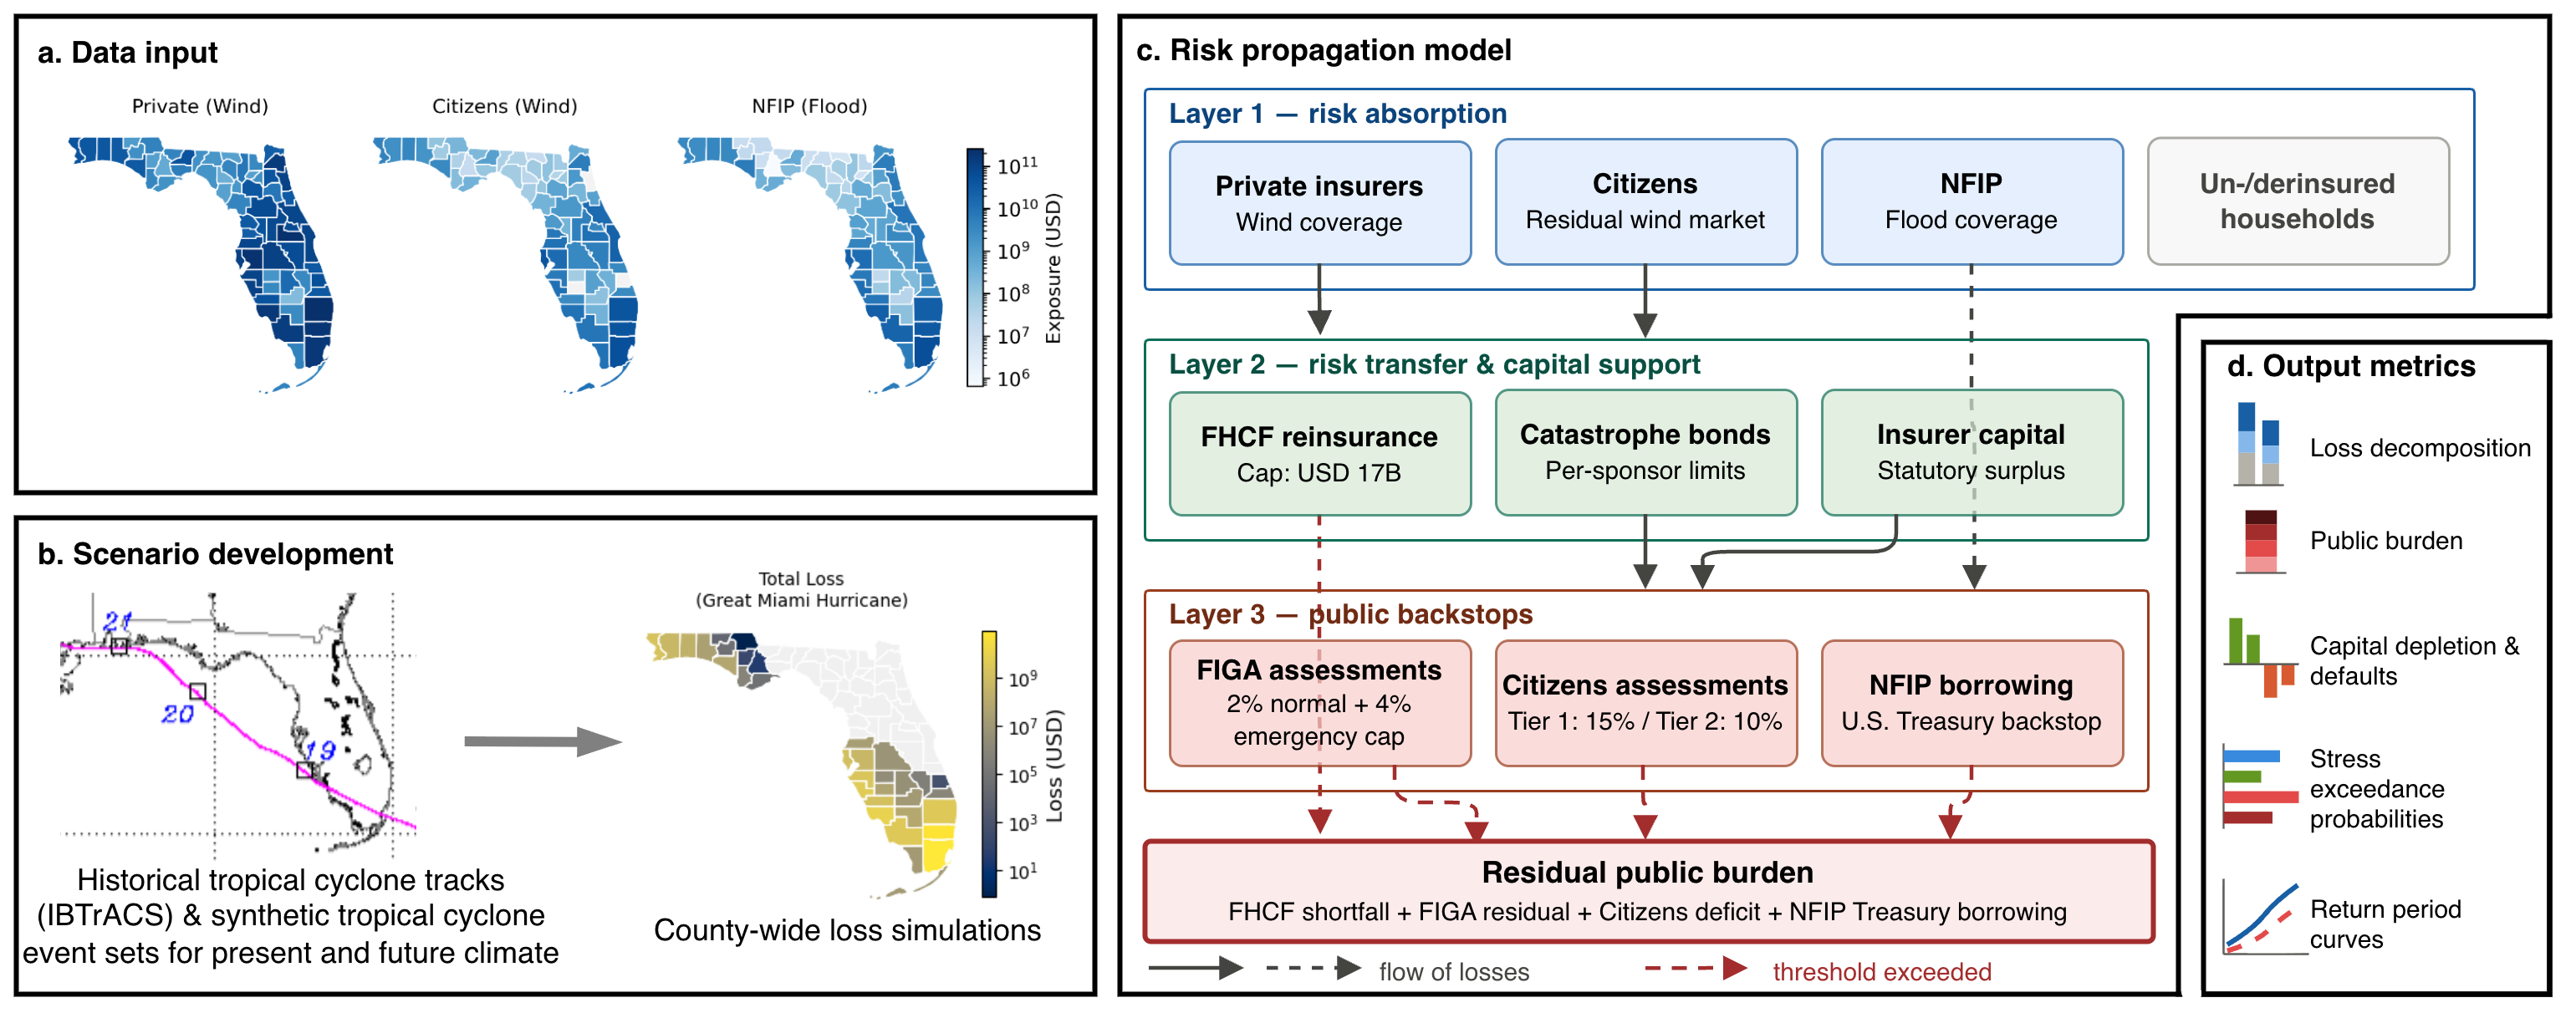
\includegraphics[width=1.0\textwidth]{figures/fig1_systemic_risk_overview_florida.png}
    \caption{\textbf{Insurance system architecture and risk propagation in the Florida homeowners' property insurance market.}
    a) County-level exposure and coverage-in-force for private wind insurers, Citizens Property Insurance Corporation (Citizens), and the U.S. National Flood Insurance Program (NFIP), together with the policy terms, capital positions, and contractual constraints used as model inputs.
    b) Illustrative example of the hazard-to-loss estimation for a single event. The track of the 1926 Great Miami Hurricane (from IBTrACS; left) is translated into county-level wind and flood loss estimates using the specified economic exposure (right). For clarity, only this one historical track is shown; the probabilistic analysis additionally draws on large synthetic tropical cyclone event sets representing present-day and future climate conditions (Methods), which are not displayed here.
    c) Loss propagation through three sequential layers. (1) risk absorption by private insurers, Citizens, the NFIP, and un-/under-insured households; (2) risk transfer and capital support via the Florida Hurricane Catastrophe Fund (FHCF; statewide seasonal cap USD 17B), catastrophe bonds, and insurer statutory surplus; and (3) public backstops, comprising Florida Insurance Guaranty Association (FIGA) assessments (2\% normal plus up to 4\% emergency), Citizens' two-tier assessments (Tier 1 up to 15\%, Tier 2 up to 10\%), and NFIP Treasury borrowing, which together determine the residual public burden. Solid arrows denote the flow of losses; dashed black arrows indicate the flow of losses that bypass one layer; dashed red arrows indicate losses transferred once an institutional threshold or statutory cap is exceeded.
    d) Main output metrics are color-coded to the model layer in (c) that generates them. They include loss decomposition, public burden by backstop, insurer capital depletion and defaults, stress exceedance probabilities, and return period curves, evaluated under single, sequential, and probabilistic event scenarios.}
    
\label{FigOverview}
\end{figure*}


\subsection{Hurricane hazards and economic losses}\label{DataTCtracks}\label{MethodsHazModel}\label{MethodsWindFloodSplit}
Historical tropical cyclone (TC) tracks come from IBTrACS \cite{knapp_international_2010}. Synthetic tracks are generated with the statistical-dynamical MIT TC model \cite{emanuel_statistical_2006,emanuel_hurricanes_2008}, using ERA5 for the present climate and five CMIP6 global climate models (GCMs) for future conditions. We retain tracks passing within 150~km of Florida's coast. The ERA5 reference spans 1980--2023. Each GCM supplies a historical reference for 1995--2014 and projections for 2041--2060 and 2081--2100. Track generation and frequency calibration are described in Supporting Text~S2.

We calculate economic losses with CLIMADA \cite{aznar-siguan_climada_2019}. The Holland wind model \cite{holland_revised_2008} converts each track into a wind field on a grid of 120~arc-seconds. LitPop distributes 2020 GDP values using population and nightlight intensity \cite{eberenz_asset_2020}. We combine this exposure with the USA impact function, which relates wind intensity to relative economic damage \cite{eberenz_regional_2021}. Although wind provides the predictor, the function was calibrated against total cyclone losses and incorporates average rainfall and surge contributions. It does not resolve damage to individual residential buildings. We aggregate the resulting losses to counties before applying the insurance model.

Wind and flood losses enter different insurance programs. To separate them, we use county contributions derived from the multi-hazard damage regression of Gori et al.\ \cite{gori_sensitivity_2025,gori_tropical_2025}. For each realization, we rescale these contributions to a sampled wind share, centered at 84.6\% for the synthetic catalog. Historical scenarios use separate wind share distributions. Flood loss is the remainder. This approach partitions aggregate economic losses rather than independently simulating rainfall and surge damage. Sea-level rise is not included. Supporting Text~S2 gives the attribution equations, rescaling procedure, and wind share means for historical storms.

\subsection{Insurance exposure and loss allocation}\label{DataInsuranceMarket}\label{MethodsRiskAbsorption}
We assign county wind exposure to private insurers and Citizens using their total insured values. Private exposure comes from Florida Hurricane Catastrophe Fund (FHCF) reports, and Citizens supplies its own county records \cite{fhcf_coverage_2024,citizens_policies_in_force_2024}. Within the private market, we allocate exposure among the largest 100 insurers in proportion to their statewide residential premiums \cite{floir_marketshare_2024}. Applying the same shares across counties preserves statewide market composition but removes differences in insurers' geographic concentration. Statutory surplus reported for individual insurers and affiliated groups, obtained through S\&P Capital IQ, defines available capital. Supporting Text~S1 documents these inputs and their reference dates.

We represent the insured share of wind losses with a Beta(4,6) distribution, with mean 0.40. Its calibration uses Florida insurance losses, NFIP payments, and reconstructed economic losses for 2017--2024 (Supporting Text~S3). The empirical ratio has total economic loss in its denominator, whereas the model applies the fraction to wind loss. We therefore use it as an allocation assumption, not a direct measurement of residential wind coverage. Insured wind losses are divided among insurers by county exposure. The remaining losses stay outside the modeled insurance system. These losses cannot be assigned entirely to households because the economic exposure includes more than residential property.

For flood, FEMA's NFIP Residential Penetration Rates dataset estimates the proportion of residential structures insured in each county \cite{fema_nfip_penetration_2025}. The denominator is the estimated residential stock from the National Structure Inventory. We combine rates inside and outside Special Flood Hazard Areas using their shares of that stock. We apply the resulting county rate to flood losses and cap claims at county NFIP coverage-in-force \cite{fema_nfip_redacted_policies_v2_2024}. This assumes that insured structures carry the same share of losses as their share of the county's residential stock. Supporting Text~S3 details the calculation and its limitations.

\subsection{Risk transfer, capital depletion, and institutional backstops}\label{MethodsRiskProp}\label{MethodsRiskTransferCapital}
The FHCF reimburses participating wind insurers for eligible claims above a retention, the amount they must first absorb themselves. Recoveries depend on each insurer's chosen reimbursement percentage and contract limit \cite{fhcf_annual_report_2023,fhcf_coverage_2024}. We constrain combined recoveries to the modeled seasonal capacity of USD~17~billion and reduce them proportionally when demand exceeds that amount. Catastrophe bonds provide additional recoveries when the relevant loss thresholds are reached, up to their payout limits \cite{artemis_catbond_2024}. We represent them as covers for a single occurrence without reinstatement. Private reinsurance treaties are not included.

We subtract recoveries from insured wind losses and apply the remaining claims to statutory surplus. An insurer with negative surplus may receive support from an affiliated group, subject to the group's available capital and an eligibility rule. Insurers still in deficit after this support are classified as insolvent. This calculation represents the exhaustion of modeled capital, rather than a prediction of a regulatory liquidation decision. Supporting Text~S4 specifies the contracts, capital accounting, and group support rule.

The Florida Insurance Guaranty Association (FIGA) covers claims following private insurer insolvency through assessments on surviving insurers. We compare the combined deficit with one year's modeled assessment capacity, comprising 2\% normal and 4\% emergency assessments of surviving insurers' written premiums \cite{flastat,figa_assessments}. Any excess remains a residual financing requirement. For Citizens, losses remaining after recoveries draw on its statutory surplus \cite{citizens_annual_statement_2024}. Two assessment tiers then provide financing, limited in the model to 15\% of Citizens' premium base and 10\% of the statewide property premium base \cite{citizens_assessments}. We record the deficit remaining after both tiers. These assessments spread costs among insurers and policyholders. They are not state expenditure. The calculation does not capitalize future assessment streams or represent financing through bonds backed by those streams.

NFIP claims draw on a national fund balance of USD~3.441~billion \cite{crs_nfip_fund_balance_2025}. Claims above this amount are recorded as Treasury borrowing requirements. We do not represent NFIP reinsurance or enforce the statutory borrowing ceiling. This output therefore measures the additional financing required under the modeled claims, including amounts that may exceed existing borrowing authority. Losses elsewhere in the United States are outside the analysis. Together, these rules identify where insured losses exceed available resources. The thresholds can cause residual requirements to rise faster than gross losses as additional financing layers are exhausted. Full equations and parameter values are provided in Supporting Text~S4 and Table~S9.

\subsection{Simulation design and experiments}\label{MethodsFutureClim}\label{MethodsPolicy}\label{MethodsBuildingCodeClimate}
We apply the model to four historical storm footprints and three constructed sequences, with 200 Monte Carlo realizations per scenario. These are stress tests under the specified exposure and market conditions, rather than reconstructions of historical losses. Sequential scenarios reduce exposed asset values after the first storm but do not model changes in vulnerability or recovery. The probabilistic assessment samples storms with replacement according to catalog frequencies to form 10,000 synthetic seasons for each climate dataset, including seasons with no events. We apply the financial model once to each season's aggregated losses, starting with the same capital in every season. Supporting Text~S5 describes the sampling and aggregation.

For SSP2--4.5, we estimate each GCM's change in a risk metric between its future and historical simulations. We add the median change across the five GCMs to the ERA5 baseline. This combines the baseline estimate with the modeled climate signal rather than using GCM projections directly as future risk levels. The same procedure applies to expected annual losses and exceedance probabilities. Additional scenario comparisons are documented in Supporting Text~S5.

We also vary market structure, insurance coverage, and physical losses in separate experiments. Market contraction increases Citizens' share from 15\% to 25\%, with changes in exposure and capital. Expanded coverage raises the assumed insured wind fraction from 40\% to 60\% and flood penetration from approximately 11\% to 30\%, alongside changes in premiums, capital, and Citizens' share. The mitigation experiment reduces wind losses by 30\% and flood losses by 25\% before insurance allocation. These prescribed reductions represent the effect of lower damage, not an engineering model of particular building standards. Finally, we vary loss reductions to identify those that offset mid-century climate effects on each metric. Supporting Text~S5 gives the scenario settings and the offset calculation.

\subsection{Outcome metrics and amplification}\label{MethodsOutput}
We track uninsured losses, insured claims, insurer defaults, and the largest insurer deficit. Institutional stress is measured against each modeled capacity. We also compare NFIP claims with Florida premium income and aggregate burden with Florida GDP. Table~S2 defines all indicators.

The public burden indicator combines FIGA and Citizens residual deficits and NFIP borrowing requirements. FHCF reimbursement shortfalls are tracked separately: tracing the model shows that whenever an FHCF shortfall is not absorbed by an insurer's own remaining capital, it already appears inside that insurer's or Citizens' deficit, so adding it to the sum would double-count that portion. The indicator records stress across financing channels whose costs need not fall on the same actors, and it should not be interpreted as a forecast of government expenditure.
% RESOLVED (Earth's Future revision, correction register item C1). Verified
% by tracing fl_risk_model.runner (capital depletion is applied to net wind
% loss, after FHCF and cat-bond recovery) and confirmed with deterministic
% fixtures (fl_risk_model/tests/earths_future/test_accounting_fixtures.py).

Annual exceedance probabilities are the fraction of simulated seasons above a specified threshold. Return periods express the inverse annual exceedance probability. In Table~\ref{TabProbRPvalues}, the public burden return levels are now the empirical quantiles of the season-level sum of its components, and total loss return levels remain independently ranked marginal quantiles. Figure~\ref{FigLossPublicBurdenScaling} compares these two series; it is not a claim about paired outcomes within individual seasons for the loss side, though the public burden series is now itself a genuine season-level aggregate. Supporting Text~S6 gives the estimator and the quantile convention.
% RESOLVED (correction register item R1). Table 1 and the amplification
% figure were recalculated from season-level sums using
% scripts/earths_future_revision/section5_return_periods.py on the archived
% ERA5 baseline (10,000 seasons); see the correction register for the
% numerical effect (10y/100y amplification: 43.9x submitted -> 31.1x
% corrected; power-law exponent 1.64 -> 1.51).

\subsection{Uncertainty and model evaluation}\label{MethodsUncertainty}
We sample the insured wind fraction, wind share, and county insured values, the latter with a coefficient of variation of 0.15. Other financial parameters remain fixed within each experiment. Table~S8 separates sampled inputs from fixed assumptions and climate model variation.

We examine sensitivity to the insured wind fraction over values from 0.1 to 0.5 (Table~S6) and to NFIP flood-loss allocation using three configurations that assign county flood losses through the baseline structure-weighted rate, entirely within Special Flood Hazard Areas, or entirely outside them (Supporting Text~S3). A 300-season by 50-parameter-draw nested design was also used to compare hazard-driven and parameter-driven variance; because the 300 seasons were selected to span the loss distribution rather than sampled at random, this design does not evaluate uncertainty in all structural assumptions and is not the basis for the robustness claims in this paper.

We use 1,000 bootstrap resamples of the ERA5 seasons to characterize sampling uncertainty. Future estimates additionally report the 10th to 90th percentile range of changes across GCMs. These ranges represent different sources of uncertainty. Comparisons with normalized historical losses and Florida's institutional experience provide consistency checks, rather than formal validation. In particular, the low modeled FHCF recovery for Irma reflects its assumed wind share and differs from observed reimbursements. Supporting Text~S6 describes the checks and their scope.


\section{Results}
\subsection*{Stress testing the insurance system with historical and sequential events}
We examine how extreme losses are distributed across households, insurers, and public backstops, using four historically damaging TCs affecting Florida: the Great Miami Hurricane (1926), the Lake Okeechobee Hurricane (1928), Hurricane Andrew (1992), and Hurricane Irma (2017). These four storms span distinct hazard profiles and historical eras, ranging from intense wind over the modern Miami metropolitan area to inland and statewide flooding, and they are among the most damaging TCs in Florida's history. We selected them as recognizable, high-consequence analogues for stress testing. Throughout, these named storms denote stylized stress-test scenarios: each is a historical hazard footprint evaluated on 2024 exposure and insurance market conditions, not a reconstruction of the original event or of its realized losses. To probe how the system responds to temporally clustered events, we also construct sequential scenarios that combine these footprints within a single season: a paired scenario, in which two different storm scenarios occur in succession (Great Miami followed by Andrew), and repeated-event scenarios, in which the same storm scenario occurs twice within the same season (Great Miami twice; Irma twice). Modeled total losses (\SITabIII) fall within the range of published normalized estimates (Supplementary Material Table 2 in Mueller et al., 2025 \cite{muller_normalized_2025}.\medskip

Across all scenarios, approximately 60--75\% of losses remain uninsured or underinsured (Fig.~\ref{FigScenario}a), with the highest shares occurring in flood-heavy events affecting inland areas with low flood insurance penetration (Fig.~\ref{FigOverview}a, right-most panel). Public burden --- residual losses propagated through the insurance system to public institutions after private capital and statutory backstop capacities are exhausted --- reaches approximately USD~12~billion for Hurricane Andrew, USD~18~billion for the Lake Okeechobee Hurricane, and USD~26~billion for the Great Miami Hurricane. Sequential events generate public burdens of USD~50--65~billion, exceeding the sum of individual-event burdens: a nonlinear amplification of public costs reflecting institutional thresholds and payout caps. By contrast, Hurricane Irma losses are largely absorbed by the initial insurance layers (public burden of USD~0.2~billion). These differences reflect the magnitude of insured losses reaching the backstops rather than total losses alone. Although Irma's total losses are large, they fell disproportionately on flood-exposed areas of low insurance penetration, so much of the loss remained with uninsured households and only a small residual propagated to the public backstops. Although the FHCF only reaches its statutory cap for Great Miami-scale or sequential events, FIGA, Citizens, and the NFIP accrue deficits in most scenarios that would require multiple years of premium income to recover (\SITabIII, stress ratios). \medskip\medskip

\begin{figure*}[htb!]
    \centering
    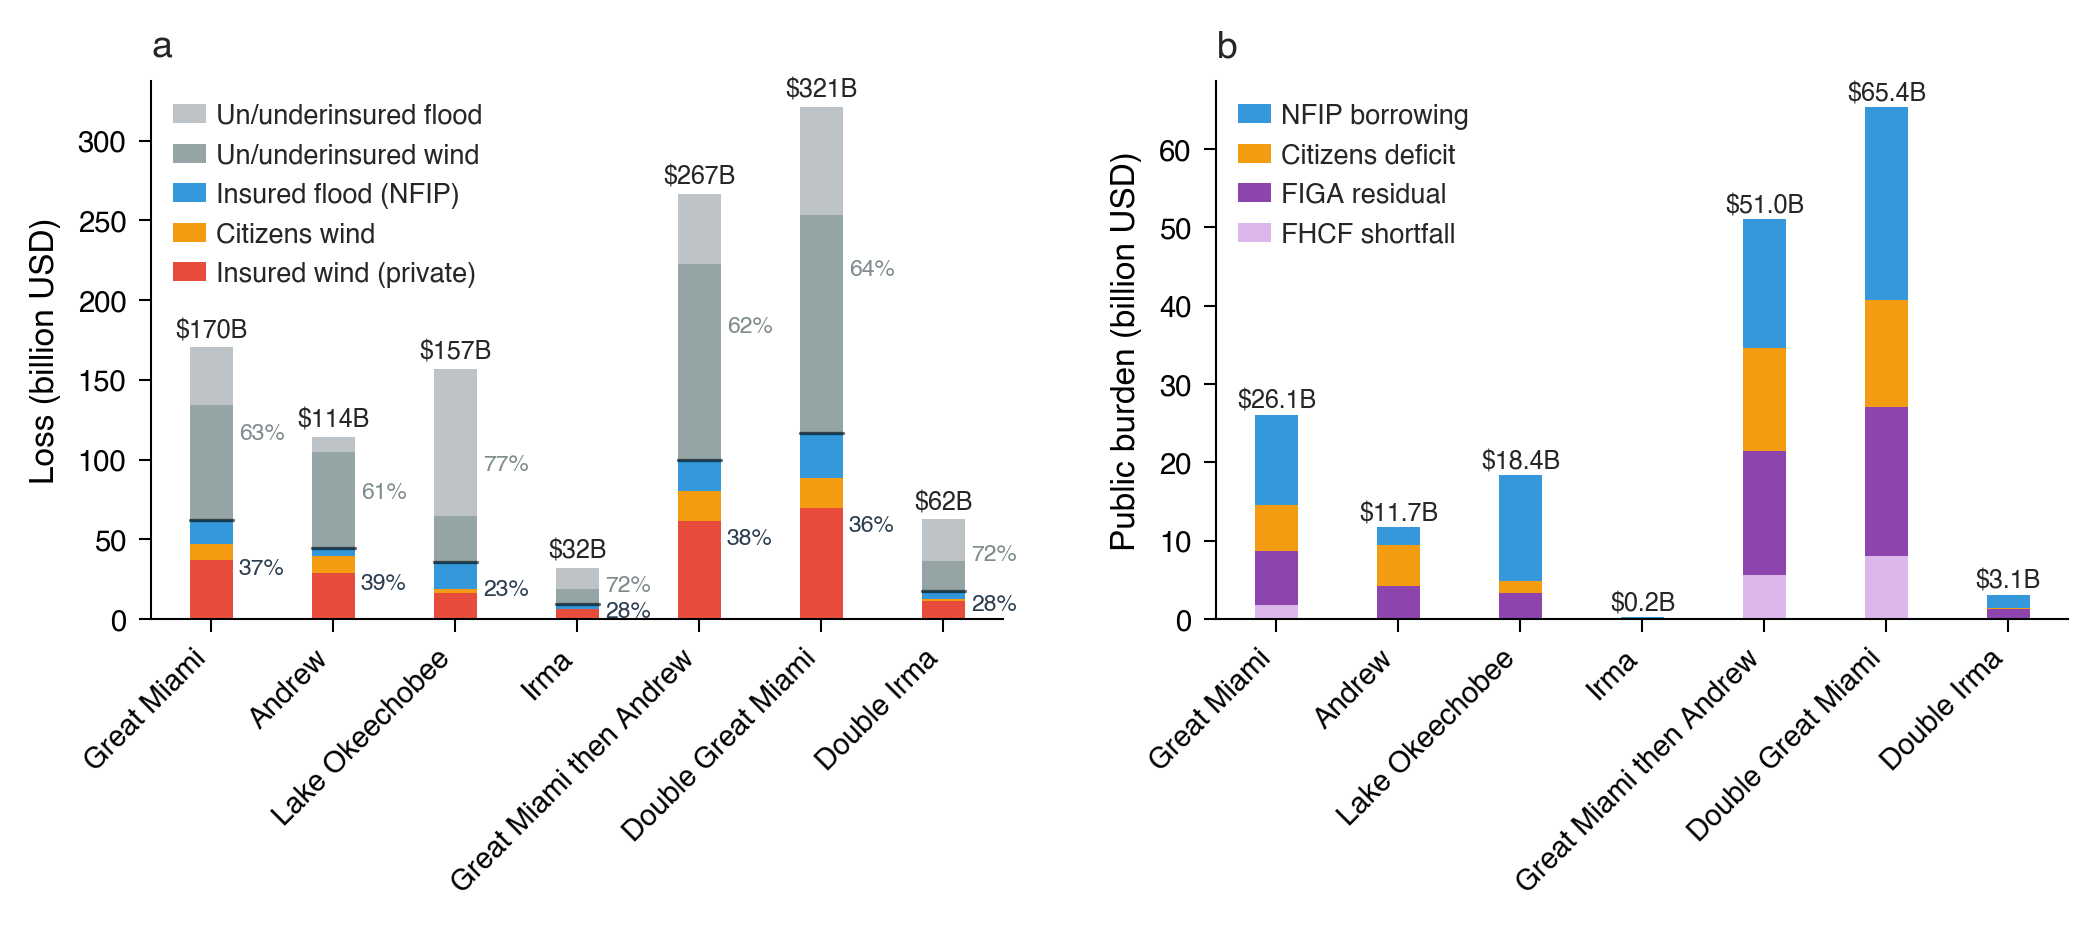
\includegraphics[width=1.0\textwidth]{figures/fig_loss_institutional_stress.png}
    \caption{\textbf{Loss decomposition and public burden across historical and sequential TC scenarios.}
    a) Decomposition of total losses across insured wind (private market and Citizens), insured flood, and uninsured or underinsured losses. The black horizontal line indicates the split between insured and uninsured losses, with corresponding shares shown numerically.
    b) Public burden after exhaustion of private insurer capital and risk transfer mechanisms, apportioned across key public backstops.
    Total loss and public burden values (billion USD) are shown above each bar.
    All values are shown for single and sequential-event scenarios; a complete tabulation, including uncertainty ranges, is provided in \SITabIII.
    Named storms denote stylized hazard footprints evaluated on 2024 exposure and insurance market conditions, not reconstructions of the original events or their realized losses.}
\label{FigScenario}
\end{figure*}

\subsection*{Probabilistic assessment of systemic insurance risks}
Moving beyond individual scenarios, we quantify systemic insurance risk probabilistically using a catalog of \num{10000} simulated TC seasons (Section~\hyperref[MethodsHazModel]{Hurricane hazards and economic losses}). Table~\ref{TabProbRPvalues} places the scenario-based stress tests into a probabilistic context by reporting seasonal return period estimates under present-day climate conditions. A total seasonal loss comparable to the Great Miami Hurricane ($\approx$\,USD~170\,billion) corresponds to a return period of approximately 35 years under present-day climate and exposure, while the sequential-event scenarios examined above approach the magnitude of a 100-year season.\medskip

Moreover, the probabilistic results reveal pronounced nonlinear amplification of public burden with increasing loss severity (Fig.~\ref{FigLossPublicBurdenScaling}). For each return period, we compare the estimated total public burden with the corresponding estimate of total seasonal loss. If public burden increased proportionally with total losses, the relationship would follow a constant-share reference line. Instead, public burden rises much more steeply, scaling approximately with the 1.51 power of total loss over the return period range shown. While total seasonal losses increase by approximately a factor of nine between the 10-year and 100-year levels (USD~39.5 to 357.2~billion), total public burden increases by more than a factor of thirty (USD~1.9 to 58.6~billion; Table~\ref{TabProbRPvalues}). This supralinear scaling reflects exhaustion of private insurer capital, activation of institutional thresholds, and binding payout caps that shift an increasing share of losses to public and quasi-public backstops in the tail of the distribution. In most seasons, the layered insurance architecture absorbs losses without imposing any public burden: about 86\% of simulated seasons carry none, and burden emerges only in more severe seasons, beyond approximately the 7-year return level.
% CORRECTED (Earth's Future revision, register item R1+C1): total public burden is now the empirical return level of the season-level sum of FIGA residual, Citizens deficit, and NFIP Treasury borrowing (a non-overlapping definition; see Table~\ref{TabProbRPvalues} note and \SIMethodsI\ Text~S4/S6). The submitted version summed four separately-estimated marginal component quantiles, including the FHCF shortfall, which overlaps with FIGA/Citizens deficits for insurers whose FHCF cap-driven shortfall contributed to their own default. See docs/earths_future_revision/correction_register.md items R1 and C1 for the full derivation.\medskip

Across return periods, FIGA residuals constitute the largest and fastest-growing component of public burden. In a 100-year season, FIGA residual losses (USD~32.8~billion) account for the majority of the total public burden, exceeding both Citizens deficits (USD~17.2~billion) and NFIP  borrowing (USD~10.3~billion). FIGA remains the dominant channel through which losses enter quasi-public balance sheets across the full range of return periods considered. FHCF shortfalls (reported separately below) are comparatively limited and occur primarily in more extreme seasons; they are not added into total public burden because, when they are not absorbed by an insurer's own remaining capital, they already appear inside that insurer's or Citizens' deficit.\medskip

\begin{table}
\centering
\caption{Loss decomposition and public institutional burden across return periods.
Return period (RP) estimates are shown for total losses, their decomposition across insured and uninsured components, and the resulting public and quasi-public institutional burden. Total public burden is the empirical return level of the season-level sum of FIGA residual, Citizens deficit, and NFIP Treasury borrowing; FHCF shortfall is shown separately as an upstream diagnostic of FHCF capacity stress because it is not additive with the other three components (\SIMethodsI\ Text~S4/S6). Public burden reflects residual financial obligations borne by public backstops after exhaustion of private insurer capital and risk transfer mechanisms.}
\label{TabProbRPvalues}

\small
\setlength{\tabcolsep}{4pt}

\begin{tabular}{lrrrrrrr}
\toprule
& \multicolumn{7}{c}{\textbf{Return period [years]}} \\
\cmidrule(l){2-8}
\textbf{Metric (USD B)} &
\textbf{10} &
\textbf{25} &
\textbf{50} &
\textbf{100} &
\textbf{250} &
\textbf{500} &
\textbf{1000} \\
\midrule
\multicolumn{8}{l}{\textit{Loss decomposition}} \\
Total loss                     & 39.5 & 146.9 & 246.4 & 357.2 & 563.9 & 628.0 & 738.0 \\
Insured wind -- private        & 11.6 & 41.8 & 69.7 & 103.2 & 155.2 & 198.4 & 214.3 \\
Citizens wind                  & 1.8 & 6.8 & 14.5 & 22.1 & 35.6 & 53.6 & 62.9 \\
Insured flood -- NFIP          & 0.9 & 3.7 & 7.4 & 13.7 & 26.1 & 37.6 & 50.3 \\
Un/underinsured wind           & 19.8 & 71.8 & 125.9 & 183.1 & 257.6 & 321.1 & 392.1 \\
Un/underinsured flood          & 3.9 & 15.1 & 28.4 & 47.1 & 87.3 & 112.7 & 141.7 \\
\midrule
\multicolumn{8}{l}{\textit{Institutional stress}} \\
Total public burden (corrected)& 1.9 & 15.5 & 33.3 & 58.6 & 99.1 & 136.1 & 163.4 \\
FHCF shortfall (diagnostic)    & 0.0 & 0.0 & 6.5 & 13.7 & 20.8 & 26.8 & 29.6 \\
FIGA residual                  & 1.0 & 9.2 & 19.2 & 32.8 & 54.9 & 72.8 & 80.6 \\
Citizens deficit               & 0.7 & 4.5 & 9.9 & 17.2 & 29.3 & 47.3 & 57.2 \\
NFIP Treasury borrowing        & 0.0 & 0.2 & 4.0 & 10.3 & 22.7 & 34.1 & 46.8 \\
\bottomrule
\end{tabular}
% CORRECTED (register item R1+C1): "Total public burden" row is now the
% empirical return level of the season-level sum of FIGA + Citizens + NFIP
% (all 10,000 ERA5 seasons, quantile q=1-1/RP, linear interpolation),
% reproducible via scripts/earths_future_revision/section5_return_periods.py.
% The submitted row summed the four marginal quantile rows below it
% (including FHCF shortfall), which does not equal the quantile of the
% season-level sum and double-counts FHCF shortfall already embedded in
% FIGA/Citizens deficits. FHCF shortfall is retained as a diagnostic row
% (statewide unrecovered reimbursement demand against the $17B cap) and is
% not part of the "Total public burden" sum.
\end{table}

\begin{figure*}[htb!]
    \centering
    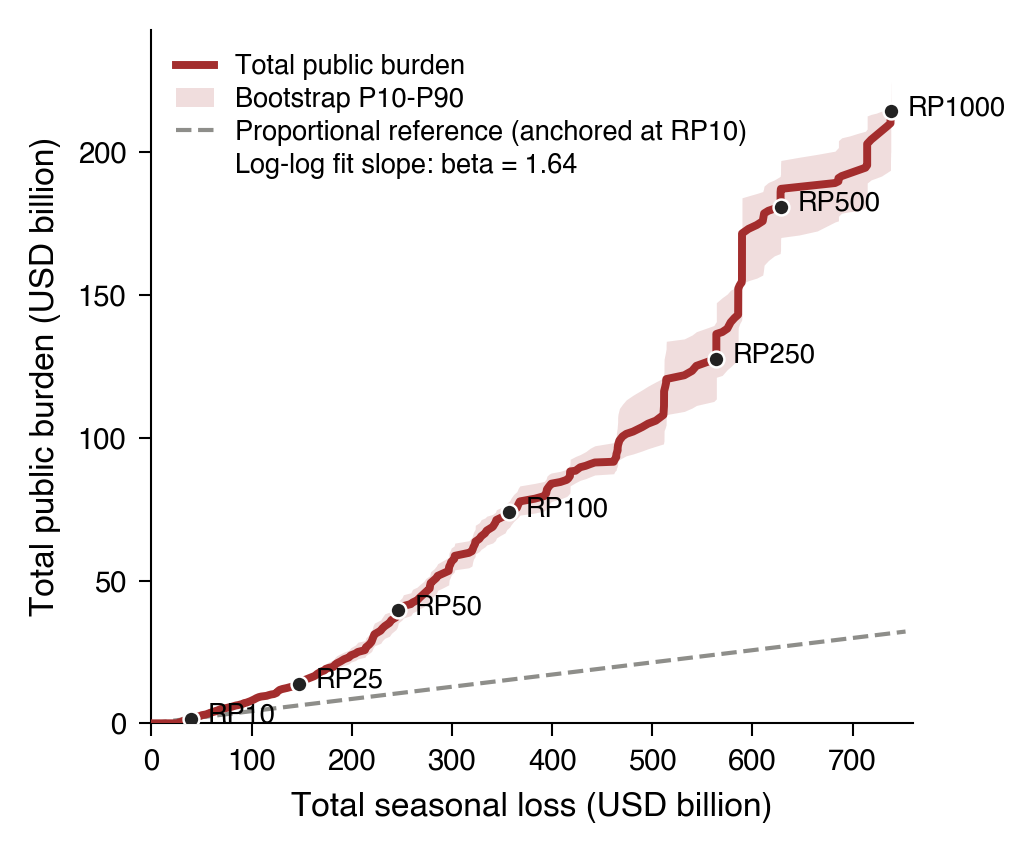
\includegraphics[width=0.5\textwidth]{figures/fig_public_burden_scaling_linear.png}
    \caption{\textbf{Supralinear scaling of public burden with seasonal loss.} Total public burden plotted against total seasonal loss for present-day climate and the 2024 market configuration, based on 10,000 simulated tropical cyclone seasons. Points show estimates at the return periods (RPs) reported in Table~\ref{TabProbRPvalues}. The dashed line shows a proportional, constant-share reference anchored at the 10-year RP; the public burden curve lies above this reference, indicating that public burden increases faster than proportionally with total loss (log-log slope $\beta \approx 1.51$). Total loss return levels are marginal quantiles; total public burden return levels are quantiles of the season-level sum of its components, so the curve compares a marginal quantile series with a season-aggregate quantile series rather than paired per-season outcomes (\SIMethodsI\ Text~S6). Total public burden is the sum of three non-overlapping institutional components: FIGA residual, Citizens deficit, and NFIP Treasury borrowing. FHCF shortfall is excluded from this sum because, whenever it is not absorbed by an insurer's own remaining capital, it already appears inside that insurer's or Citizens' deficit; it is reported separately in Table~\ref{TabProbRPvalues}. Shading shows the 10th-90th percentile bootstrap interval (1,000 resamples of whole season rows).}
\label{FigLossPublicBurdenScaling}
\end{figure*}

The probabilistic approach further allows us to assess the annual exceedance probability of systemic risk thresholds that indicate stress across different components of the insurance system (Fig.~\ref{FigProbabilistic}a, \SITabV). For the private wind insurance market, the annual probability of more than ten insurer defaults is 11.4\%, while the probability that the single largest company deficit exceeds USD~1~billion is 7.2\%.

For public and quasi-public institutions, the annual probability of exceeding capacity or statutory thresholds differs across entities. The probability that the FHCF reaches its statewide seasonal payout cap is 0.8\%, whereas the probabilities of FIGA and Citizens exceeding their respective assessment capacities are 13.6\% and 9.5\%. For the NFIP, the probability that annual losses exceed twice its annual premium income is 5.0\%. These results mirror the scenario-based findings in Fig.~\ref{FigScenario}, highlighting comparatively greater vulnerability of FIGA, Citizens, and the NFIP relative to the FHCF.

Finally, we relate the aggregate public burden to the economic scale of Florida. Using the corrected, non-overlapping public burden definition (FIGA plus Citizens plus NFIP), the annual probability that total public burden exceeds 1\% of Florida's GDP is 3.7\%, while the probability of exceeding 10\% of state GDP is 0.1\% (down from 0.13\% under the submitted four-component definition; \SIMethodsI\ Text~S6).

\begin{figure*}[htb!]
    \centering
    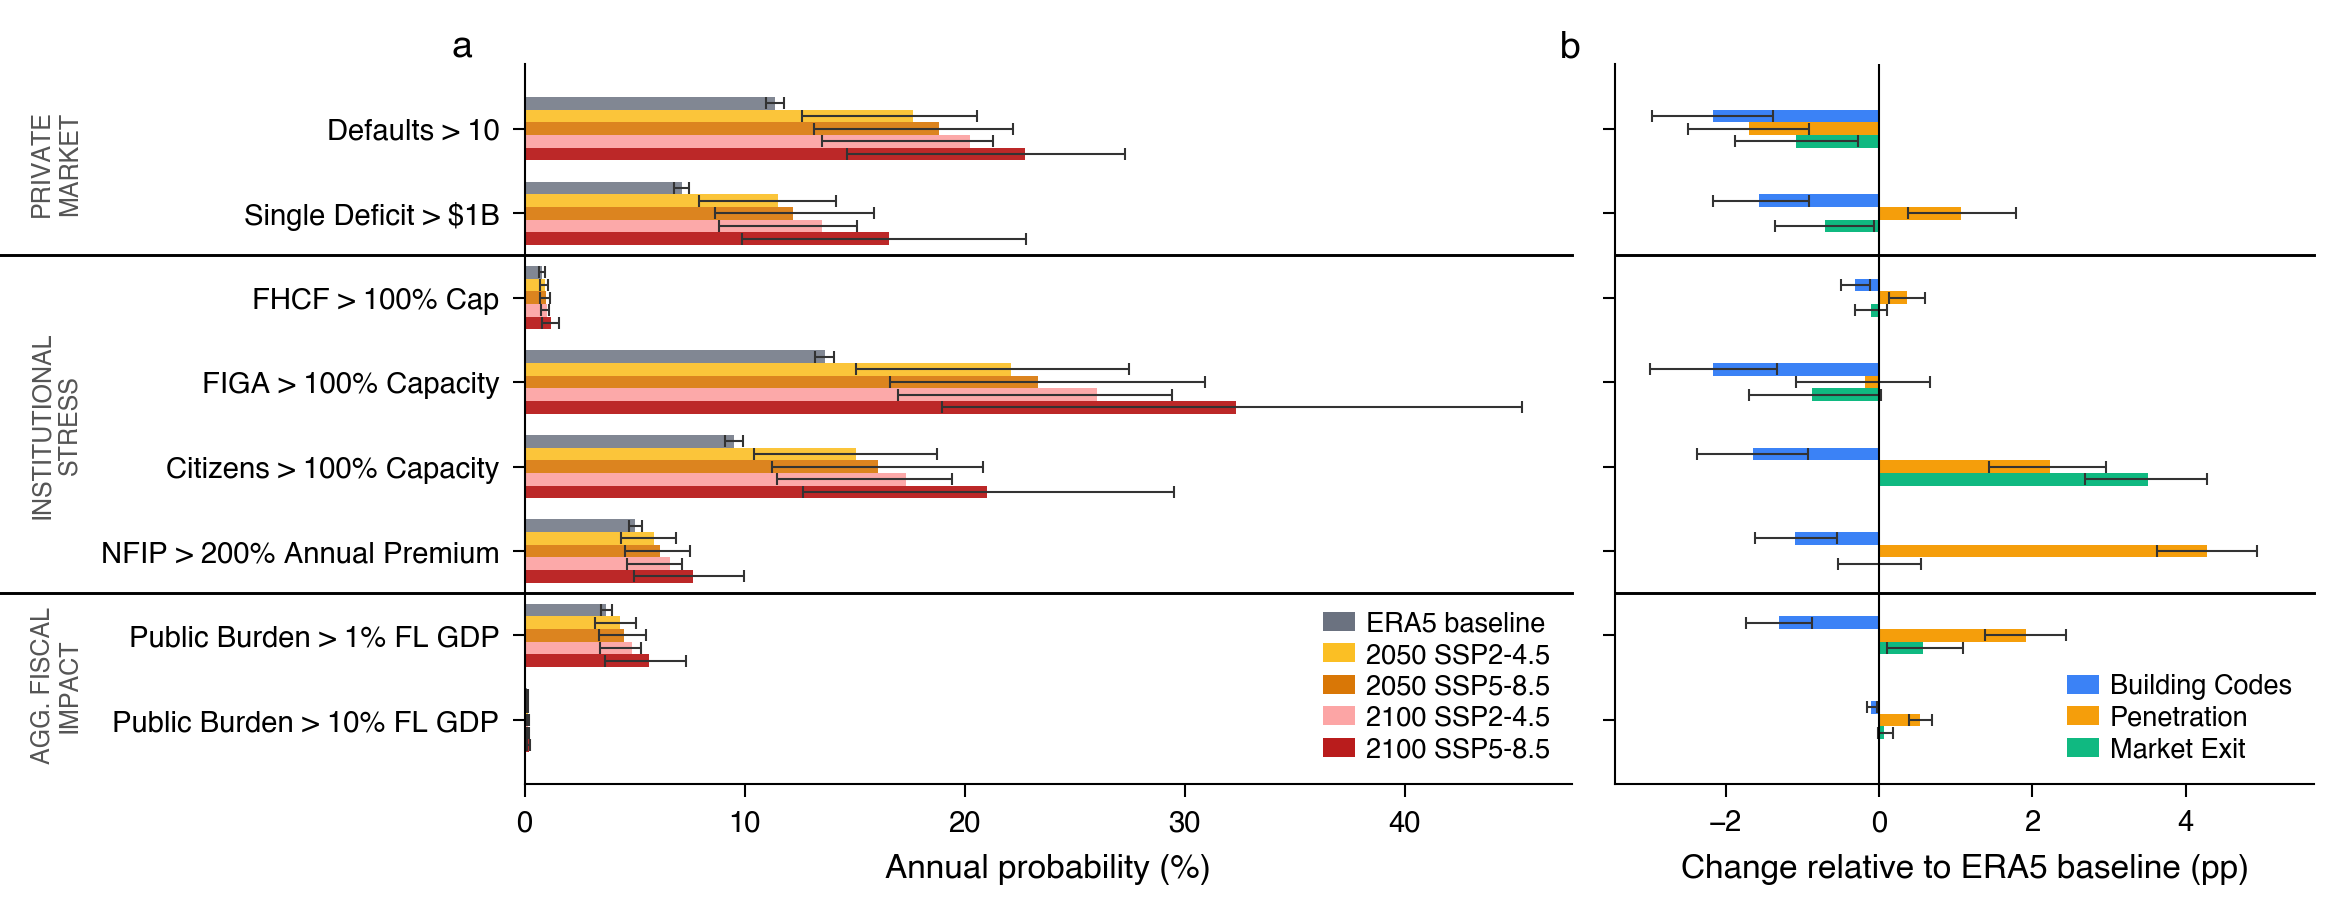
\includegraphics[width=1.0\textwidth]{figures/fig_combined_climate_policy_systemic_risk.png}
    \caption{\textbf{Probabilistic assessment of systemic insurance risks under future climate scenarios and stylized policy interventions.} Annual exceedance probabilities of predefined systemic stress thresholds across the private insurance market (top), public and quasi-public entities (middle), and aggregate fiscal impact measured as total public burden relative to Florida's GDP (bottom). (a) Absolute annual exceedance probabilities under present-day and future climate conditions. Shown are results for the ERA5 baseline climate (grey), mid-century SSP2-4.5 (yellow) and SSP5-8.5 (orange), and end-of-century SSP2-4.5 (pink) and SSP5-8.5 (red). Bars show mean annual exceedance probabilities corresponding to the median climate-induced risk change across the GCMs used for tropical cyclone track set generation (Section~\hyperref[MethodsFutureClim]{Simulation design and experiments}), based on \num{10000} simulated tropical cyclone seasons; error bars indicate the 10th--90th percentile range across the full GCM ensemble. (b) Changes in annual exceedance probabilities relative to the ERA5 baseline configuration under three stylized policy scenarios: private insurer market exit (green), increased insurance penetration (orange), and strengthened building codes (blue). Values represent percentage-point changes under present-day hazard conditions. Bars show mean changes based on \num{10000} simulated tropical cyclone seasons, with error bars indicating the 10th--90th percentile. Positive values indicate an increase in the probability of exceeding the corresponding stress threshold relative to baseline; negative values indicate a reduction.}
\label{FigProbabilistic}
\end{figure*}

\subsection*{Systemic risk probabilities increase with climate change}\label{ResultsClimate}
We next evaluate how projected changes in TC hazard alter systemic insurance risk, holding exposure, capital positions, and regulatory parameters at present-day values. Projections span mid-century (2041--2060) and end-of-century (2081--2100) under SSP2-4.5 and SSP5-8.5 emission scenarios. Future changes are estimated using a multi-model delta approach: ensemble-median changes in each risk metric across five CMIP6 simulations are added to the ERA5-based present-day baseline (Section~\hyperref[MethodsFutureClim]{Simulation design and experiments}). Throughout, the SSP and period labels identify the corresponding GCM-ensemble hazard deltas rather than a specific emissions pathway, since different emissions trajectories can produce similar deltas. The changes reported below therefore isolate the response of the present-day insurance architecture to climate-driven shifts in the TC loss distribution.\medskip

Under mid-century scenarios (2041-2060), expected annual total losses approximately double relative to present-day conditions, and expected public burden increases by a factor of approximately three (\SITabIV). Exceedance probabilities of several systemic stress thresholds increase across the private market and post-insolvency channels (Fig.~\ref{FigProbabilistic}, \SITabV). The annual probability of more than ten insurer defaults rises from 11.4\% under present-day conditions to 17.7\% (SSP2-4.5) and 18.8\% (SSP5-8.5).\medskip

Post-default and residual-market mechanisms exhibit particularly strong amplification. The probability that FIGA exceeds its statutory assessment capacity increases from 13.6\% to 22.1--23.3\%, while Citizens exceeds its assessment capacity with probabilities rising from 9.5\% to 15.1--16.1\%. In contrast, the probability that the FHCF reaches its statewide payout cap remains at or below 1\% across scenarios, and the probability that NFIP annual losses exceed twice premium income increases only modestly (from 5.0\% to 5.9--6.1\%).\medskip

Uncertainty across climate models is substantial but does not alter the qualitative direction of change (\SITabV). Under 2050 SSP5-8.5, the probability that FIGA exceeds capacity ranges from 16.6\% to 30.9\% across the GCM ensemble, compared with 13.2--14.1\% at baseline, with similar spreads for private insurer defaults and Citizens deficits. Differences between emission scenarios widen by end-of-century but remain smaller than the inter-GCM range.
At the aggregate level, the annual probability that total public burden exceeds 1\% of Florida's GDP increases modestly from 3.7\% to 4.3--4.5\% by mid-century, while exceedance of 10\% of GDP remains rare.\medskip


\subsection*{Systemic risks with evolving markets and insurance policies}
We next evaluate how changes in market structure and insurance policies modify systemic risk under present-day hazard conditions. The three stylized interventions represent dynamics currently discussed in policy and industry debates: private market contraction and expansion of residual markets following recent insolvencies and insurer withdrawals \cite{hemmati_growing_2025,CDI2024AnnualReport,kousky_evolution_2024};
expansion of insurance penetration to reduce protection gaps \cite{kousky_insurance_2024}; and strengthened building codes and retrofitting initiatives aimed at reducing physical losses \cite{wolf_are_2025,ibhs_fortified_standard_2025}. Each intervention modifies a distinct layer of the insurance system architecture while holding all other model components constant (Section~\hyperref[MethodsPolicy]{Simulation design and experiments}). \medskip

\paragraph{Private insurer market exit}
We model a contraction of the private wind market that increases Citizens' market share from 15\% to 25\% of total insured value, corresponding to a 10\% shift of exposure from private insurers, of which 85\% transfers to Citizens and 15\% becomes uninsured.
Under this scenario, the annual probability of more than ten private insurer defaults declines by about 1.1 percentage points relative to the ERA5 baseline (Fig.~\ref{FigProbabilistic}b, \SITabV), reflecting the reduced exposure and insured loss volume within the private market. However, systemic stress shifts toward residual market mechanisms. The probability that Citizens exceeds its assessment capacity increases by about 3.5 percentage points, while exceedance of the FHCF statewide payout cap remains nearly unchanged (\SITabV). Expected total public burden rises from USD~2.7~billion to USD~3.1~billion (\SITabIV), and the probability that total public burden exceeds 1\% of Florida's GDP increases by around 0.6 percentage points (Fig.~\ref{FigProbabilistic}b, \SITabV). 

\paragraph{Insurance penetration increase}\label{ResPenetration}
We increase wind (from 40\% to 60\%) and flood (from 11\% to 30\%) penetration rates, with insurer surplus and NFIP premium volumes scaling proportionally to insured exposure.
While expanded coverage reduces uninsured losses from USD~12.1~billion (combined wind and flood) under baseline conditions to USD~7.8~billion (\SITabIV), its systemic effects are heterogeneous. Several indicators of stress in public or quasi-public institutions increase under higher insurance penetration. Most notably, the annual probability that NFIP losses exceed 200\% of annual premium income increases by 4.3 percentage points relative to the ERA5 baseline (Fig.~\ref{FigProbabilistic}b, \SITabV), despite the proportional expansion of the premium base --- reflecting both the geographic concentration of the new exposure and the supralinear growth of tail losses relative to mean losses under correlated risk. The probability that Citizens exceeds its assessment capacity increases by 2.3 percentage points, and the probability that total public burden exceeds 1\% of Florida's GDP increases by 1.9 percentage points (\SITabV). Expected public burden rises from USD~2.7~billion to USD~5.1~billion (\SITabIV).

In contrast, several indicators of stress within the private insurance market decline. The annual probability of more than ten private insurer defaults decreases by 1.7 percentage points, while FIGA exceedance decreases marginally by 0.2 percentage points (\SITabV). These patterns indicate that proportional scaling of capital and premium income does not automatically preserve institutional resilience when insured loss volumes increase (Section~\hyperref[MethodsPolicy]{Simulation design and experiments}). 

\paragraph{Building code improvement}
We reduce wind-related losses by 30\% and flood-related losses by 25\% relative to baseline vulnerability before allocation across institutional layers.
Exceedance probabilities decline consistently across private, residual, and public components (Fig.~\ref{FigProbabilistic}b, \SITabV). The annual probability of more than ten private insurer defaults decreases by 2.2 percentage points relative to the ERA5 baseline, FIGA exceedance decreases by 2.1 percentage points, and Citizens capacity exceedance decreases by 1.6 percentage points. The probability that total public burden exceeds 1\% of Florida's GDP declines by 1.3 percentage points (\SITabV). Expected total public burden decreases from USD~2.7~billion to USD~1.6~billion (\SITabIV). Unlike the redistribution scenarios above, structural mitigation reduces systemic stress simultaneously across all layers of the insurance architecture.
\medskip

We next quantify the building code-related loss reduction required to offset projected mid-century climate impacts (SSP2-4.5, 2041-2060) and restore systemic risk metrics to their present-day ERA5 baseline values (Fig.~\ref{FigClimateBuildingCodeSensitivity}). For the GCM ensemble median, total public burden declines approximately linearly as assumed wind and flood losses are reduced, returning to its present-day baseline at about 70\% combined loss reduction (Fig.~\ref{FigClimateBuildingCodeSensitivity}). Annual total loss responds similarly, whereas insurer defaults respond more nonlinearly, with sharper reductions beyond about 70\% loss reduction (\SIFigIII). Combined wind and flood loss reductions of 70-75\% are required to restore systemic risk metrics to baseline. The required reduction is sensitive to hazard uncertainty, ranging from 30-40\% under lower-end GCM projections to 75-80\% at the upper end. \medskip


\begin{figure*}[htb!]
    \centering
    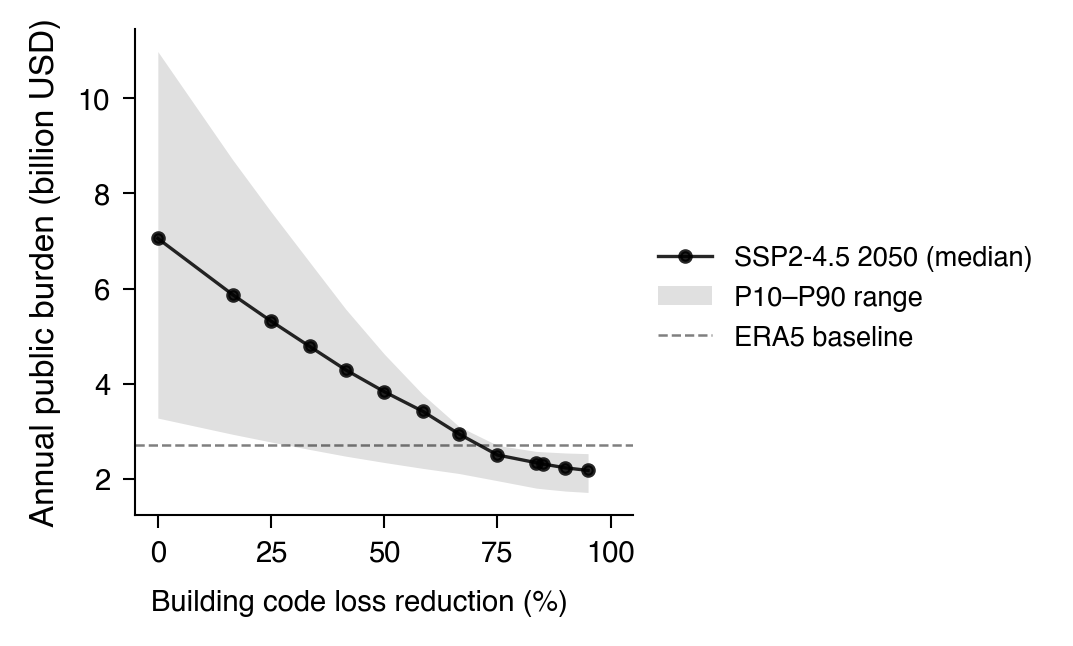
\includegraphics[width=0.5\textwidth]{figures/fig_climate_buildingcode_sensitivity_public_burden.png}
    \caption{\textbf{Sensitivity of public burden estimates to building code--related loss reductions under future climate conditions.} Sensitivity analysis showing the effect of incremental reductions in wind- and flood-related losses resulting from strengthened building codes on the estimated total public burdens under mid-century (2041-2060) SSP2-4.5 climate conditions. Solid lines indicate results for the median climate-induced risk change across the GCM ensemble, shaded bands show the 10th--90th percentile range across GCMs, and dashed lines denote the present-day ERA5 baseline. All quantities represent mean annual outcomes across \num{10000} simulated tropical cyclone seasons per climate realization. Equivalent results for annual total loss and insurer defaults are shown in \SIFigIII.}
\label{FigClimateBuildingCodeSensitivity}
\end{figure*}

\section{Discussion}
Public and quasi-public financial burdens scale disproportionately relative to primary disaster losses as institutional thresholds and capital constraints bind. Across probabilistic simulations of Florida's 2024 insurance market, total seasonal losses increase by approximately a factor of nine between 10-year and 100-year return period seasons, while total public burden increases by a factor of over forty (Table \ref{TabProbRPvalues}, Fig. \ref{FigLossPublicBurdenScaling}). Previous analyses have suggested nonlinear amplification qualitatively \cite{kousky_insurance_2024}; our probabilistic framework quantifies it.\medskip

This amplification of public burden is also unevenly distributed across institutions. The highest systemic stress falls on FIGA, followed by Citizens and the NFIP. The annual probability of exceeding institutional capacity or statutory thresholds reaches 13.6\% for FIGA and 9.5\% for Citizens (Fig. \ref{FigProbabilistic}a). In contrast, the FHCF remains comparatively resilient across baseline, climate change, and market adaptation scenarios, with a consistently low probability of reaching its statutory cap. The 13.6\% annual exceedance probability for FIGA corresponds to approximately a 1-in-7-year frequency of FIGA exhausting its assessment capacity, more than three times more frequent than Andrew-level losses, whose return period under the 2024 Florida market configuration is less than 25 years (Table~\ref{TabProbRPvalues}). Both examples are thus matters of immediate concern, not rare tail-risk scenarios.

These modeled frequencies and outcomes are broadly consistent with Florida's recent institutional history. Following the 2004-2005 hurricane seasons, Citizens' assessment capacity was effectively exceeded \cite{kousky_evolution_2024}. Its 2005 deficit, on the order of USD~1.7~billion \cite{flsenate2011citizens}, was financed through multi-year post-event bonding and a statewide emergency assessment, together with a USD~715~million state appropriation (SB~1980; ch.~2006-12, Laws of Florida) \cite{flsb1980_2006}. More recently, the 2021-2023 wave of insurer insolvencies, in which at least seven residential carriers entered liquidation, triggered successive FIGA assessments: a 0.70\% assessment in 2021, a 1.3\% and a further 0.70\% assessment in 2022, and a 1.0\% multi-year emergency assessment in 2023 \cite{figa_assessments}. Over the same period, the FHCF drew down its reserves but did not breach its statutory reimbursement cap. This ordering, namely, the recurrent binding of the FIGA and Citizens mechanisms along with a resilient FHCF, mirrors the relative exceedance probabilities our study produces (FIGA 13.6\%, Citizens 9.5\%, FHCF 0.8\%). Of the storms we model, Hurricane Irma (2017) is the most recent, and the only one to occur after all the institutions we represent (Citizens, NFIP, FHCF, and FIGA) were in place, so it offers the one direct comparison. Irma was absorbed within the insurance system, with no Citizens special assessment and no exhaustion of the FHCF, in line with the small public burden of our Irma scenario (USD~0.2~billion; Table~S3). One discrepancy is worth noting explicitly: the modeled Irma scenario assumes a wind share of 50\%, well below the 84.6\% catalog default, so its modeled FHCF recovery is small, whereas the FHCF's actual Irma-related reimbursement was substantially larger, on the order of USD~6~billion, about a third of its statutory cap \cite{fhcf_annual_report_2023}. Both the modeled scenario and the historical experience remain far below the fund's capacity, so this comparison does not affect our qualitative conclusions about FHCF resilience, but it illustrates that our stress-test footprints use the study's own exposure and wind-share assumptions rather than reconstructing a specific storm's realized losses, so exact agreement with historical reimbursement is not expected. These comparisons span different market configurations, and the insolvency-driven cases reflected litigation and reinsurance costs as well as catastrophe losses. We therefore present them as qualitative corroboration that the modeled probabilities and outcomes are plausible, not as a formal out-of-sample validation. \medskip

Our results place the annual probability that public burden from hurricanes exceeds 1\% of Florida's output at 3.7\% (about once in thirty years), and the probability that it exceeds 10\% at 0.1\% (about once in a thousand years). This aggregate combines financing channels with different incidence. FIGA and Citizens deficits are residual assessment obligations that fall on surviving insurers and, ultimately, policyholders statewide; they are a private cross-subsidy within the insurance market, not government expenditure. NFIP Treasury borrowing is the one component that represents a federal financing requirement. At the 100-year return level, FIGA and Citizens deficits together (USD~50.0~billion) substantially exceed NFIP borrowing (USD~10.3~billion; Table~\ref{TabProbRPvalues}), so most of the modeled public burden is market-internal rather than a direct fiscal outlay. Because Florida's annual economic output was about USD~1.7~trillion in 2024 \cite{bea_florida_gdp_2026}, expressing this burden as a share of state GDP nonetheless indicates that climate-driven insurance losses from a single state and a single hazard can reach a fiscal scale worth tracking alongside other sources of financial-system stress, even though the FIGA and Citizens components differ in kind from a government bailout.\medskip

Because climate change, market structure, and policy interventions are evaluated within the same architecture, their effects propagate through the entire insurance system. Increasing insurance penetration with proportional capital expansion, for example, reduces private insurer stress but raises public backstop exposure: the annual probability that NFIP losses exceed 200\% of annual premium income rises by 4.3 percentage points, and Citizens capacity exceedance rises by 2.3 percentage points (Section~\hyperref[ResPenetration]{Insurance penetration increase}). Policies targeting one component of the insurance market can thus redistribute systemic risk across institutions rather than uniformly reducing it.\medskip

The market dynamics and policy interventions examined here are stylized and designed to probe systemic sensitivity rather than forecast specific outcomes. Empirical evidence suggests that conventional building codes reduce wind damage. After Florida's 2001 code revision, homes built to the updated code were about 22\% less likely to sustain wind damage and showed approximately 27\% lower damage severity~\cite{wolf_are_2025}. The enhanced, voluntary FORTIFIED standard performs substantially better, reducing insured loss frequency by 55-74\% and loss ratios by 51-72\% in Hurricane Sally~\cite{fortified_sally_2025}. Offsetting the projected mid-century (2050, SSP2-4.5) increase in systemic risk requires loss reductions of about 70-75\% under the median hazard scenario, falling to 30-40\% under lower-end projections (Fig.~\ref{FigClimateBuildingCodeSensitivity}); this range in future climate outcomes reflects differences in climate sensitivity across the underlying GCMs~\cite{meiler_uncertainties_2023}. Because these empirical estimates refer to wind damage and insurance claims from individual events, they are not directly comparable to our system-level sensitivity, which represents the combined wind-and-flood loss reduction required to restore present-day stress probabilities. As benchmarks, however, they suggest that conventional code improvements fall well short of the loss reduction required to offset median mid-century climate impacts, while the strongest documented standard delivers substantially larger reductions but remains voluntary and not yet widely adopted. Reliance on a single structural measure is therefore unlikely to suffice under stronger warming; strengthening insurance market resilience will likely require a portfolio of complementary policy and market interventions. \medskip

% Limitations
Several simplifications bound the interpretation of these results, and the majority of them bias the framework toward overstating rather than understating systemic stress (\SITabVIII). Disaggregating statewide private insurer market shares uniformly to counties, in the absence of insurer-specific county data, tends to overstate the number of simultaneous insurer defaults and the size of FIGA assessments.  Representing the FHCF as the only reinsurance mechanism omits private reinsurance, which would otherwise reduce net retained losses and, in turn, modeled defaults and FIGA assessments. The indirectly calibrated wind insured fraction, approximately 40\% in severe events, may overstate coverage in smaller events, although it aligns with observed take-up in the large-loss years that dominate systemic risk outcomes (\SIMethodsI). The 1980-2023 hazard baseline likewise tends toward somewhat higher modeled losses than industry event catalogs calibrated to longer historical records, consistent with the sensitivity of Atlantic hurricane risk estimates to baseline-period choice \cite{vecchi_changes_2021,emanuel_atlantic_2021,muller_normalized_2025}. Taken together, these choices imply that our reported magnitudes are best interpreted as upper bounds, whereas the qualitative conclusions, the supralinear amplification of public burden and its concentration in FIGA, Citizens, and the NFIP rather than the FHCF, are stable across the climate scenarios and the insured-fraction range we vary (\SITabVI). This stability claim is evaluated only for the parameters we vary; it is not a general robustness result across all structural assumptions (\SITabVIII). The principal simplification acting in the opposite direction is the omission of sea-level rise, which likely leads us to underestimate long-term flood-related systemic risk.

A second group of limitations concerns the scope of the analysis. The framework is applied to Florida and to TCs alone. Wind and flood losses are partitioned with an external multi-hazard regression that is suitable for system-level probabilistic stress testing but not for event-level attribution. For future climate scenarios, the 2024 market architecture is held fixed, so projected stress should be read as a conditional assessment of the present-day configuration rather than a forecast of how the market will evolve. \medskip

% Conclusion
By embedding probabilistic hazard realizations within a market-wide representation of insurer capitalization and public backstops, this study provides a quantitative framework for evaluating how climate-driven disaster losses propagate through insurance systems. Our results show that systemic financial exposure can increase nonlinearly with disaster losses, concentrate within specific public backstop institutions, and shift across actors in response to policy and market changes. These findings suggest that insurance market stability should be evaluated not only in terms of institutional solvency, but also in terms of whether the system reduces underlying risk, preserves access to recovery finance, and limits the transfer of losses to households, policyholders, and public institutions.\medskip

Beyond Florida, the framework developed here provides a template for stress testing other climate-exposed insurance markets. California's wildfire-prone regions \cite{abatzoglou_impact_2016} reflect the same layered risk transfer vulnerabilities shown here, and similar risk transfer markets govern disaster insurance internationally. A key priority for future research is to trace how uninsured losses propagate into housing markets, credit systems, and public finance, where emerging evidence points to climate-driven debt feedbacks at the municipal level \cite{mishra_physical_2026} and persistent protection gaps across U.S. flood markets \cite{amornsiripanitch_measuring_2025}. More broadly, system-wide stress testing can help compare policy choices, including land-use restrictions, insurance affordability measures, public backstops, and structural risk reduction, by evaluating whether they reduce underlying losses or mainly redistribute them across households, policyholders, insurers, and public institutions. Developing integrated tools that connect physical risk, insurance market structure, household protection gaps, and public finance will be essential for managing climate risk as disaster losses increasingly propagate beyond the insurance sector.\medskip


\section*{Data availability}
Data used in this study are available from the sources cited in the Methods section. Data from S\&P Capital IQ require a commercial license and are not publicly accessible.

The synthetic TC data from the MIT model are proprietary and owned by WindRiskTech L.L.C., a company that provides hurricane risk assessments to clients worldwide. Due to proprietary restrictions, these datasets are not publicly archived. However, researchers interested in accessing the data for scientific purposes can contact WindRiskTech L.L.C. at \nolinkurl{info@windrisktech.com}, subject to a non-redistribution agreement.

\section*{Code availability}
For this study, we used the Python (version 3.11+) version of CLIMADA, release v6.1.0-dev \cite{siguan_climada_2025}. Source code is openly and freely available under the terms of the GNU General Public License Version 3 \cite{aznar-siguan_climada_2019}.

Code to reproduce the results of this paper is available at a \href{https://github.com/simonameiler/systemic_insurance_risk_fl_pub/}{GitHub repository} \cite{meiler_systemic-risk_github_2026} with the identifier 10.5281/zenodo.19361128.

\bibliography{systemic_risk_fl}

\section*{Acknowledgements}
\subsection*{Funding}
SM acknowledges support from the Swiss National Science Foundation Postdoc.Mobility Fellowship (P500PN\_222189) and from the Stanford Urban Resilience Initiative. NSD acknowledges support from Stanford University. \medskip

The development of the risk propagation model underlying this study was initiated in collaboration with the Insurance Policy Advisory Committee (IPAC) of the U.S. Federal Reserve System, for which Simona Meiler developed an initial flow-of-risk modeling approach. We thank members of the IPAC Property Insurance Working Group for valuable discussions and insights that informed the conceptual design of the model. The analysis presented here represents independent academic work and does not reflect the views of the Federal Reserve System or its committees.

\subsection*{Author contributions statement}
Conceptualization: SM, SIJ\\
Methodology: SM\\
Visualization: SM\\
Datasets: SM, SIJ, KE\\
Writing - original draft: SM\\
Writing - review \& editing: SM, SIJ, KE, NSD, JWB\medskip

\subsection*{Competing interests}
All authors (SM, SIJ, KE, NSD, JWB) declare no competing interests.
Kerry Emanuel is on the board of Trusted Resource Underwriters, which insures homeowners in Florida.

\end{document}